\documentclass[a4j,11pt]{jarticle}
\usepackage{epsfig,here}
\usepackage{url}

\usepackage{color}
\usepackage{listings}

\usepackage{amsmath}

\usepackage{graphicx}

\setlength{\textwidth}{1.1\textwidth}
\setlength{\oddsidemargin}{-3pt}
\setlength{\evensidemargin}{\oddsidemargin}
\setlength{\topmargin}{10mm}
\setlength{\headheight}{0mm}
\setlength{\headsep}{0mm}

\begin{document}

\begin{center}
%\noindent
 \vspace{10mm}

{\bf {\huge 3Q 研究プロジェクト(石田研)}}
%\end{center}

\vspace{80mm}

提出日:2018年10月22日

\vspace{10mm}

系/学科/類:情報工学系

\vspace{10mm}

学籍番号:16B13354

\vspace{20mm}

{\bf {\LARGE 氏名:星野 シンジ}}
\end{center}

\newpage

\section{機械学習を用いた薬剤活性の予測}

python向けのライブラリであるdeepchemをインストールし、そのチュートリアルのひとつである「Multitask Networks on MUV」をベースにして、薬剤活性の予測を行った。

まず、チュートリアルに入っているハイパーパラメータで50回実行したときの結果は図\ref{fig1}のようになった。

\begin{figure}
	\begin{minipage}{0.50\hsize}
		\begin{center}
			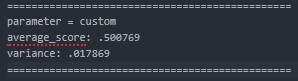
\includegraphics[width=12cm, bb=0 0 298 81]{original.jpg}
		\end{center}
	\end{minipage}
	\begin{minipage}{0.50\hsize}
		\begin{center}
			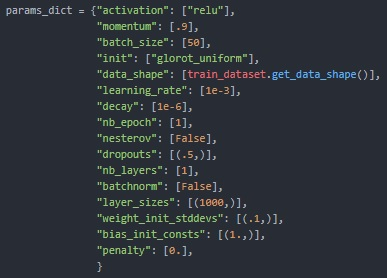
\includegraphics[width=12cm, bb=0 0 387 278]{originalp.jpg}
		\end{center}
	\end{minipage}
	\caption{デフォルトパラメーターでの実行結果}
	\label{fig1}
\end{figure}


このスコアが更に良くなるように、ハイパーパラメータを調整したい。
そこで、
もとのハイパーパラメータの変数を一つずつ変更し、十回実行したときの平均スコアがどのように変化するかを調べた。
一回実行しただけだと、偶然いい値が出る場合があるので、十回実行したスコアの平均と分散を計算した。
平均の値は、図\ref{result0}のようになった。

\begin{figure}
	\begin{minipage}{0.50\hsize}
		\begin{center}
			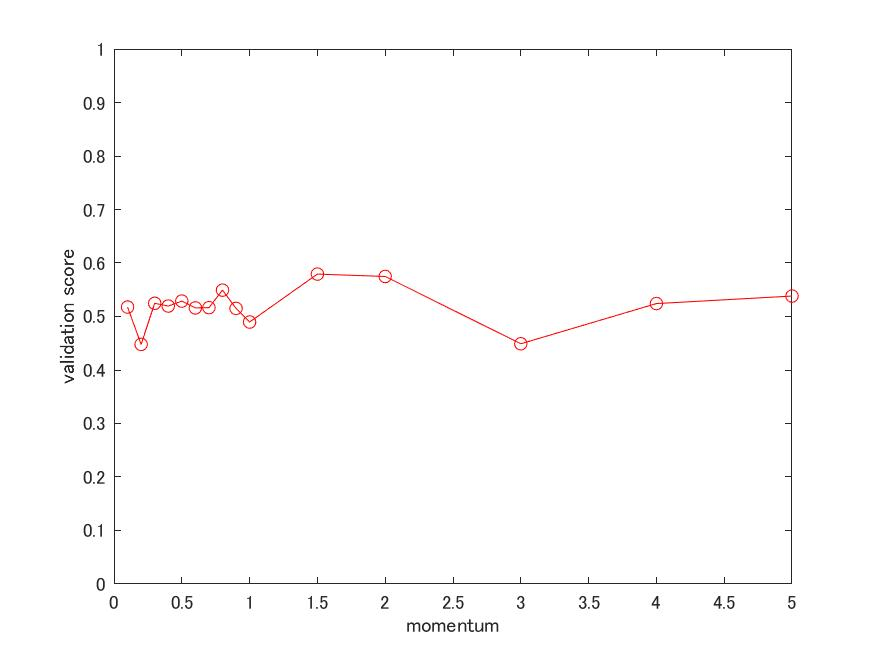
\includegraphics[width=12cm, bb=0 0 875 656]{../matlab/fig/momentum.jpg}
		\end{center}
	\end{minipage}
	\begin{minipage}{0.50\hsize}
		\begin{center}
			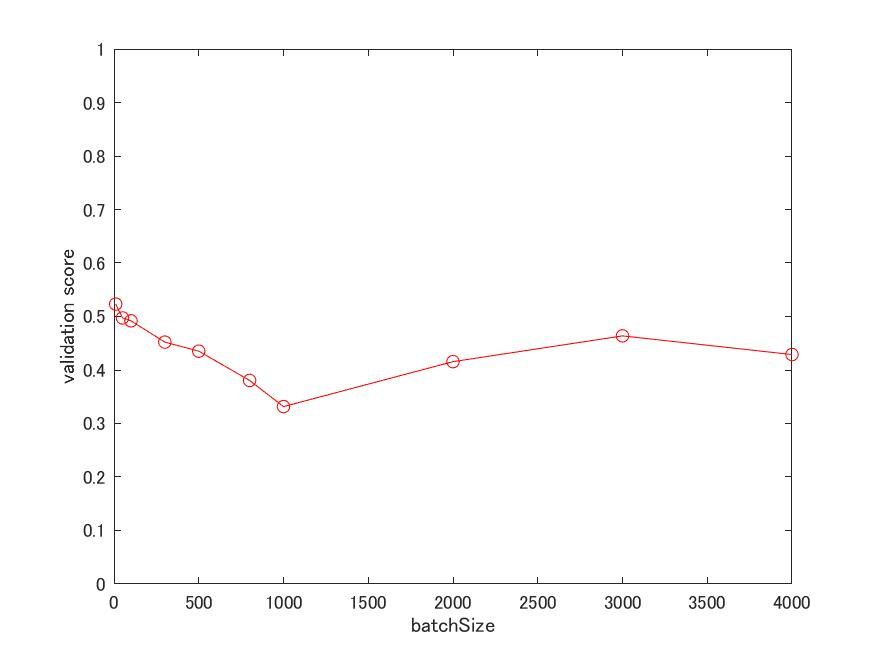
\includegraphics[width=12cm, bb=0 0 875 656]{../matlab/fig/batchSize.jpg}
		\end{center}
	\end{minipage}
	\\
	\begin{minipage}{0.50\hsize}
		\begin{center}
			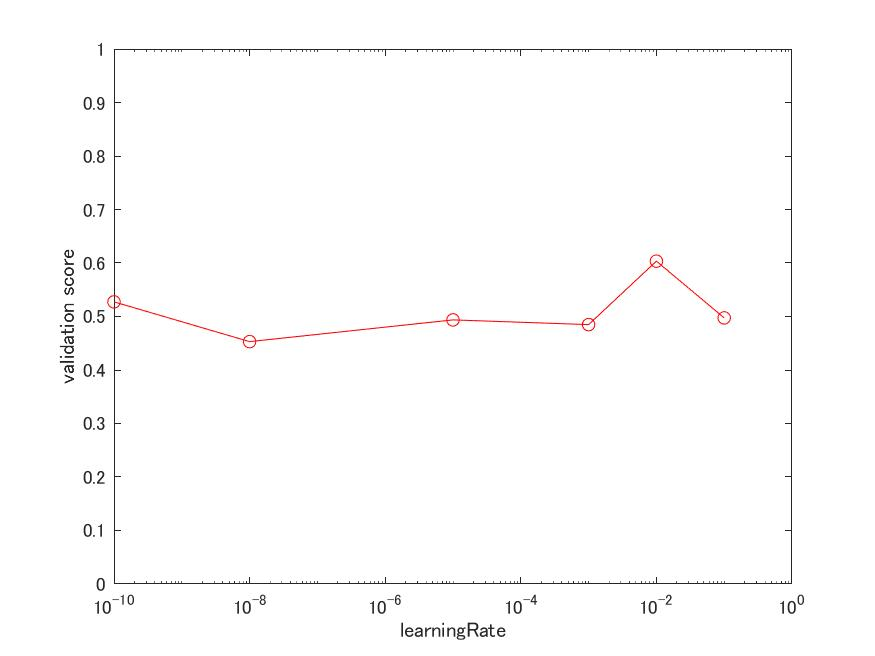
\includegraphics[width=12cm, bb=0 0 875 656]{../matlab/fig/learningRate.jpg}
		\end{center}
	\end{minipage}
	\begin{minipage}{0.50\hsize}
		\begin{center}
			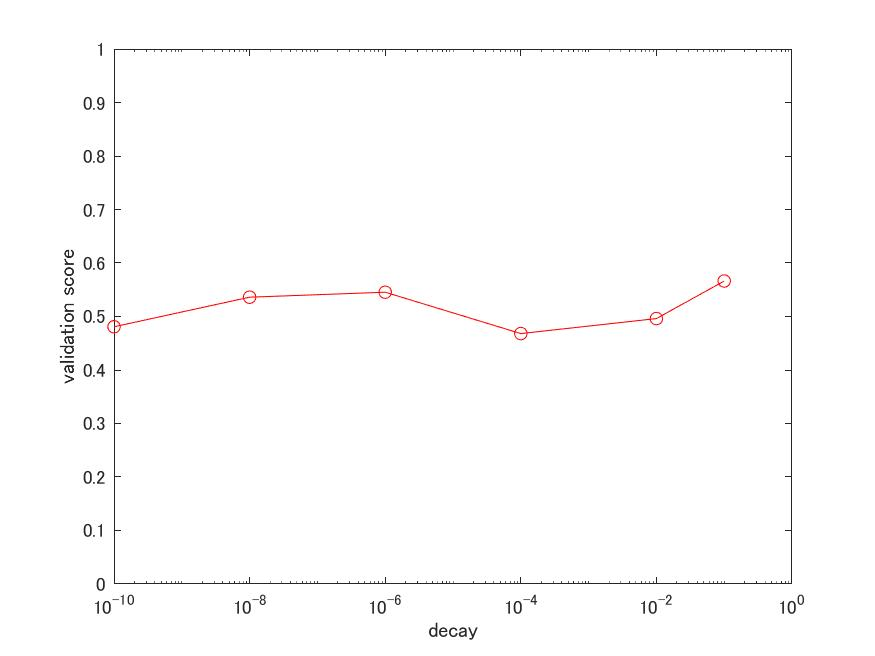
\includegraphics[width=12cm, bb=0 0 875 656]{../matlab/fig/decay.jpg}
		\end{center}
	\end{minipage}
\end{figure}
\begin{figure}
	\begin{minipage}{0.50\hsize}
		\begin{center}
			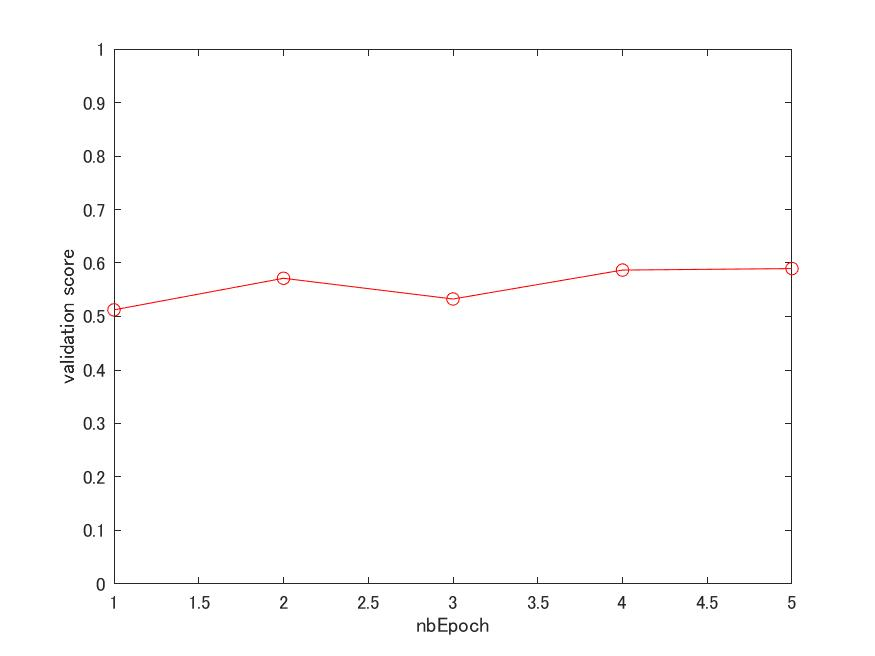
\includegraphics[width=12cm, bb=0 0 875 656]{../matlab/fig/nbEpoch.jpg}
		\end{center}
	\end{minipage}
	\begin{minipage}{0.50\hsize}
		\begin{center}
			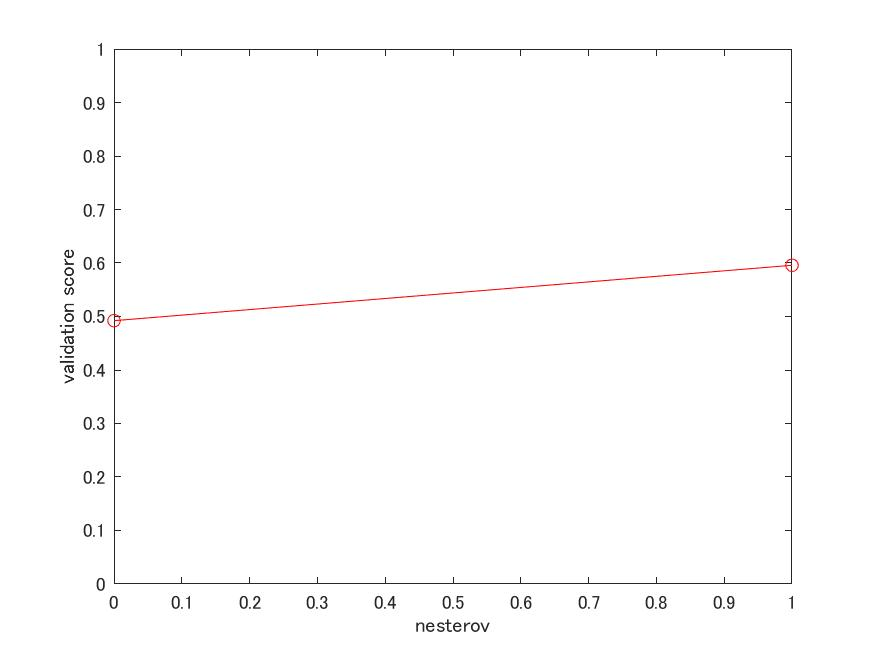
\includegraphics[width=12cm, bb=0 0 875 656]{../matlab/fig/nesterov.jpg}
		\end{center}
	\end{minipage}
	\\
	\begin{minipage}{0.50\hsize}
		\begin{center}
			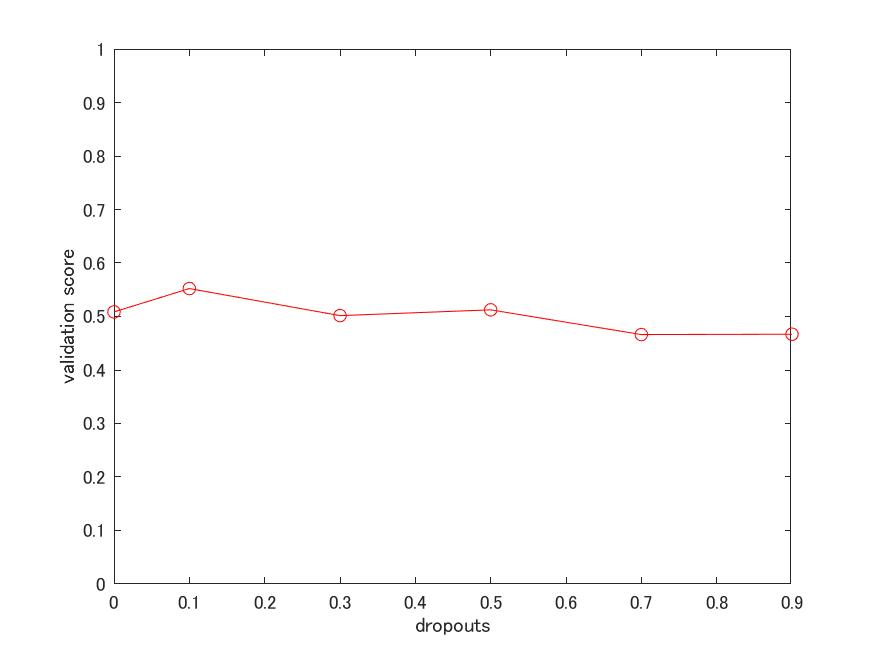
\includegraphics[width=12cm, bb=0 0 875 656]{../matlab/fig/dropouts.jpg}
		\end{center}
	\end{minipage}
	\begin{minipage}{0.50\hsize}
		\begin{center}
			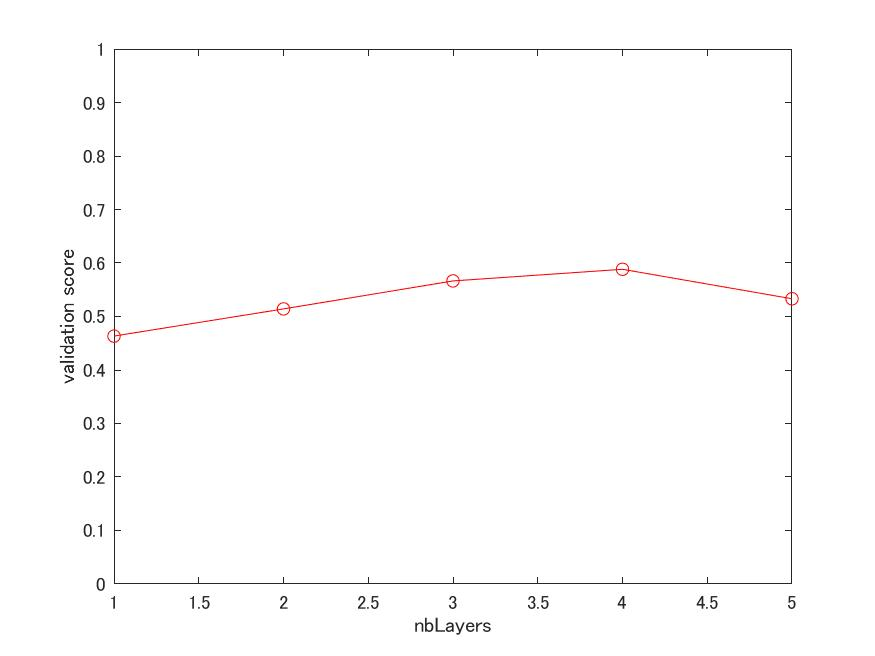
\includegraphics[width=12cm, bb=0 0 875 656]{../matlab/fig/nbLayers.jpg}
		\end{center}
	\end{minipage}
\end{figure}
\begin{figure}
	\begin{minipage}{0.50\hsize}
		\begin{center}
			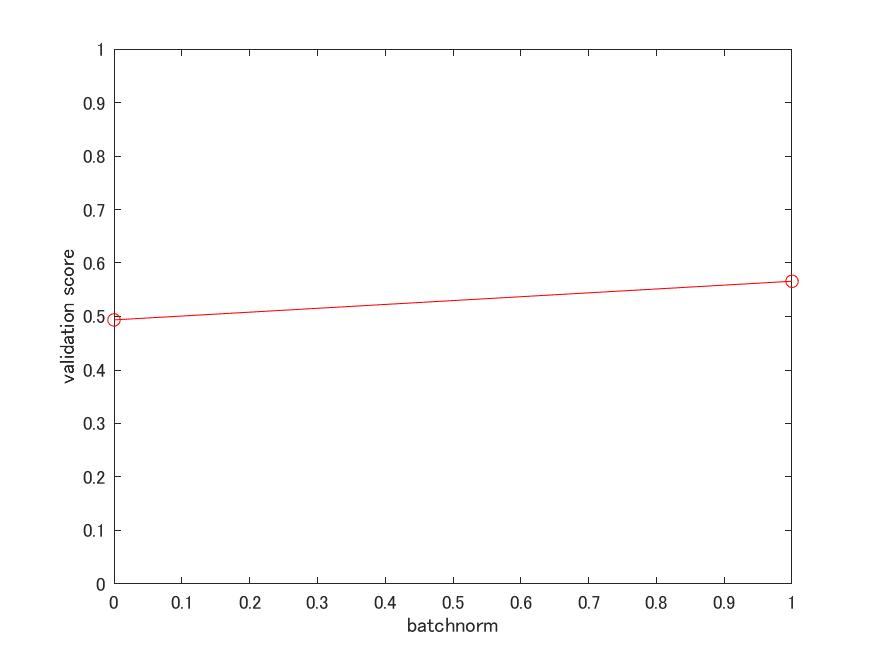
\includegraphics[width=12cm, bb=0 0 875 656]{../matlab/fig/batchnorm.jpg}
		\end{center}
	\end{minipage}
	\begin{minipage}{0.50\hsize}
		\begin{center}
			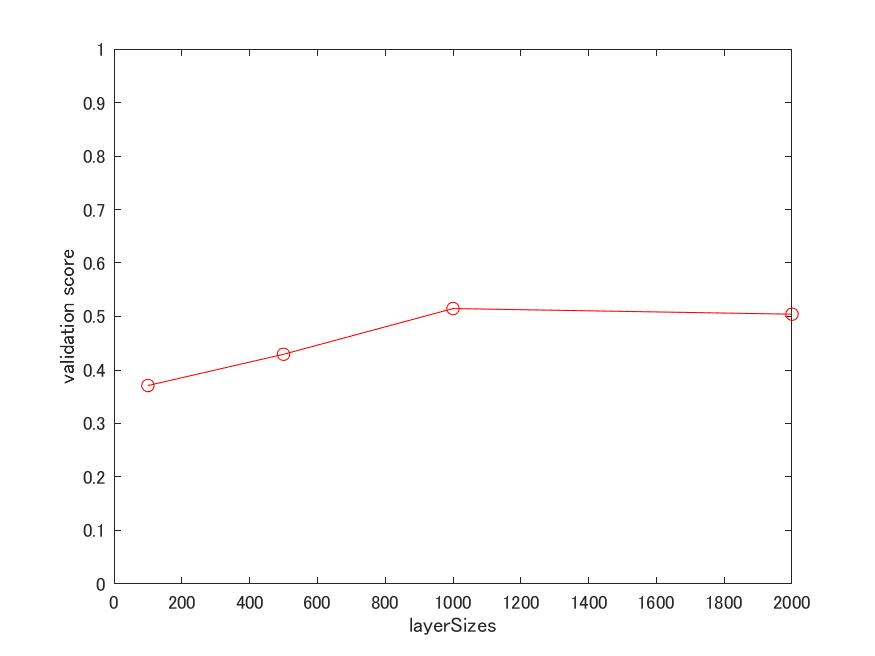
\includegraphics[width=12cm, bb=0 0 875 656]{../matlab/fig/layerSizes.jpg}
		\end{center}
	\end{minipage}
	\\
	\begin{minipage}{0.50\hsize}
		\begin{center}
			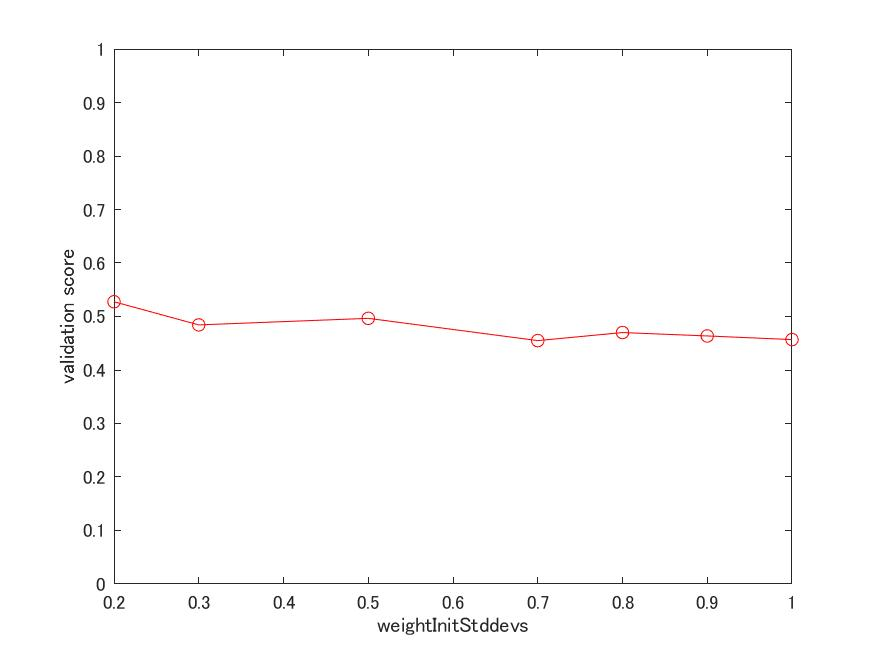
\includegraphics[width=12cm, bb=0 0 875 656]{../matlab/fig/weightInitStddevs.jpg}
		\end{center}
	\end{minipage}
	\begin{minipage}{0.50\hsize}
		\begin{center}
			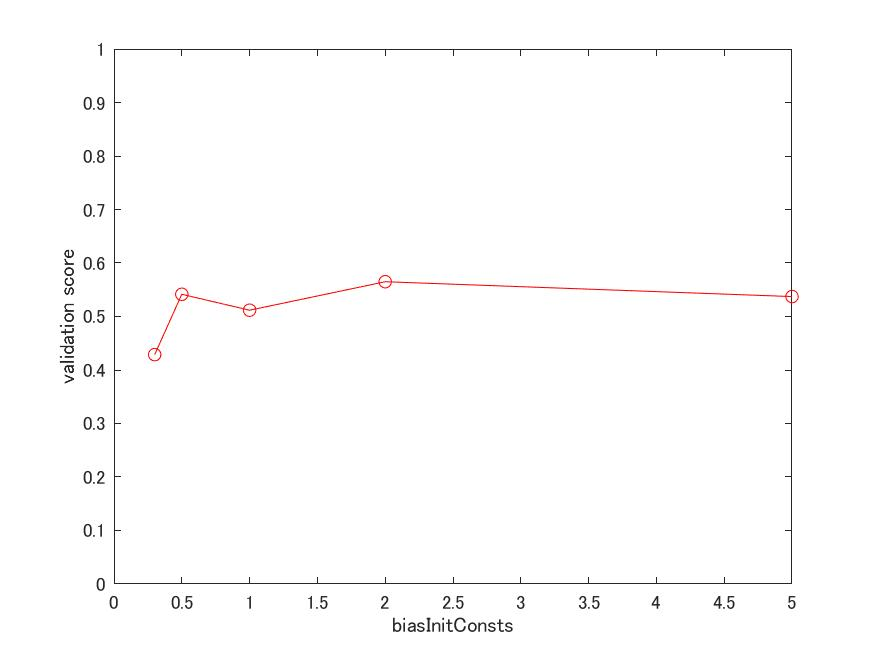
\includegraphics[width=12cm, bb=0 0 875 656]{../matlab/fig/biasInitConsts.jpg}
		\end{center}
	\end{minipage}
\end{figure}
\begin{figure}
	\begin{minipage}{0.50\hsize}
		\begin{center}
			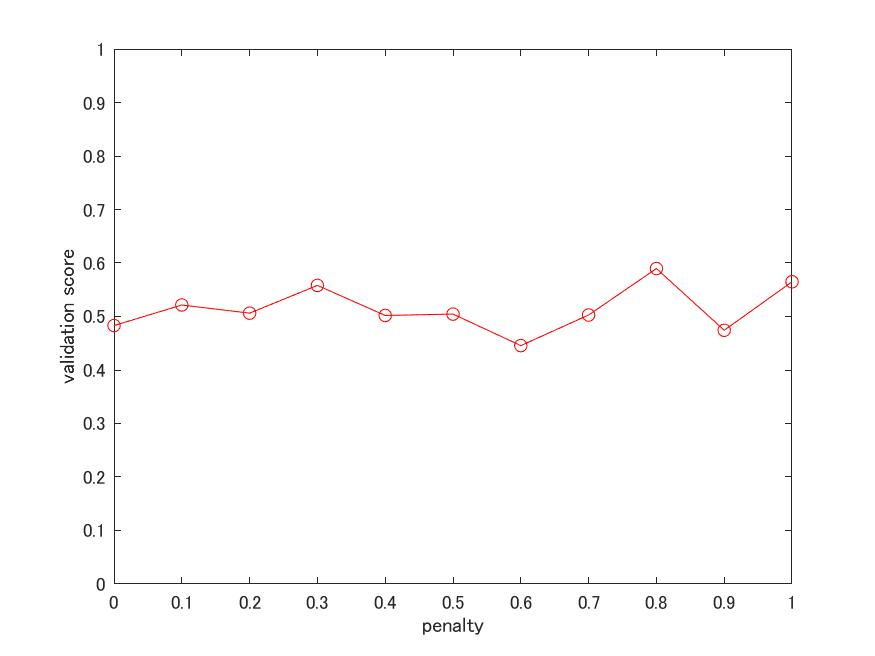
\includegraphics[width=12cm, bb=0 0 875 656]{../matlab/fig/penalty.jpg}
		\end{center}
	\end{minipage}
	\begin{minipage}{0.50\hsize}
		\begin{center}
		\end{center}
	\end{minipage}
	\caption{実験結果} \label{result0}
\end{figure}


ここまで、実験を行ったところで、より適切なハイパーパラメーターを設定できるように、
それぞれのパラメーターの意味について調べて表\ref{parameter}にまとめた。

\begin{table}[htb]
	\begin{tabular}{|l||p{10cm}|} \hline
		パラメーター名        & 説明 \\ \hline \hline
		momentum             &
エラー関数の大域的最小値を探そうとする際に、局所解を求めるようになっている。この値が大きければ大きいほど、アルゴリズムの「勢い」のようなものが大きくなり、
ある局所解が求まったとしても、より最適な解を探そうとするようになる。\cite{momentum} \\ \hline
		batch\_size           &
学習アルゴリズムが内部モデルのパラメーターを調整するまでに取り込むデータの数を示す。つまり、この数だけデータをとるごとにエラーチェックをし、修正を行う。\cite{epoch_batch}
 \\ \hline
		learning\_rate, decay &
アルゴリズムがデータから学習する際に、新しいデータの取り込みに対する
感度を示す。learning\_rateの値が大きければ大きいほど、新しいデータに強く適応するようになる。
また、データを取り込むにつれてあとから入ってくるデータの重みが小さくなっていくが、decayはその小さくなっていく速さを示す。\cite{lrd} \\ \hline
		nb\_epoch	     &
学習アルゴリズムがトレーニングデータのセットを何度学ぶかを示すパラメーター。\cite{epoch_batch}
\\ \hline
		dropout              & 過激適合を避けるために、ノード間のウェイトを均等にする必要がある。そのために、ランダムにレイヤーのノードをオフにする、
dropoutというものが行われるが、これはそれが起きる頻度を示す。\cite{dropout} \\ \hline
		nb\_layers, layer\_sizes &
ニューラルネットワークの層の数、および各層のノードの数を示す。基本的には、大きいほど性能が上がる。 \cite{layernode} \\ \hline
		weight\_init\_stddevs  &
重みの初期値を示す。これは、訓練中に調整されていく。\cite{bs} \\ \hline
		bias\_init\_consts     &
バイアスの初期値を示す。ウェイトと同じく、これも訓練中に調整されていく。\cite{bs} \\ \hline
		penalty              &
正則化を行う際の、極端なデータの重みに対するペナルティーを示す。これが大きいと、極端なデータの重みがより小さくなり、モデルに影響を与えにくくなる。\cite{regularization} \\ \hline
	\end{tabular}
	\caption{パラメーターの説明}
	\label{parameter}
\end{table}

これらの情報に基づき、一番良いパラメーターの値を分散も考慮しながら様々な組み合わせで試したところ、
図\ref{fig2}のようなパラメーターでスコアの平均をを0.613569まで上げることができた。
しかも、十回の思考での分散が0.005626ともともとのパラメーターのときよりも小さくなっているので、安定して6割程度の制度を得た。
この時、とくに影響のあったパラメーターは、nb\_epochとnb\_layersであった。
epochは大きめに設定してトレーニングを繰り返すことを行ったために制度が上がったと考える。
また、layersを適切な値にすることによって1レイヤーの時より複雑なモデルになったが、過学習を起こすほどで
はないようになったと考える。
それぞれのパラメーターのスコアへの影響を考えると、
これよりも精度を上げるためには、レイヤーの数とそれぞれのレイヤーでのノードの数をさらに最適化することに注目したほうが
いいと考えた。

\begin{figure}
	\begin{minipage}{0.50\hsize}
		\begin{center}
			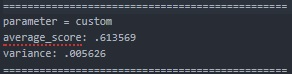
\includegraphics[width=12cm, bb=0 0 292 74]{optimal1.jpg}
		\end{center}
	\end{minipage}
	\begin{minipage}{0.50\hsize}
		\begin{center}
			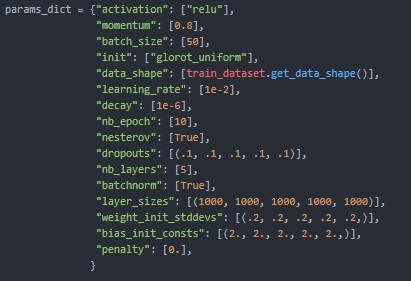
\includegraphics[width=12cm, bb=0 0 411 281]{optimal1p.jpg}
		\end{center}
	\end{minipage}
	\caption{パラメーターとその実行結果}
	\label{fig2}
\end{figure}



層の数を増やした状態で、さらに層ごとに変数を変化させたらどうなるかを実験したかったが、
計算に時間がかかりすぎるので行わなかった。
しかし、手動でいくつか試してみたところさらに良いパラメーターの組み合わせを見つけることができたので、
図\ref{optimal2}にパラメーターとその実行結果を示しておく。
層とノードの設定はそのままにし、ほかのパラメーターを変化させてみたが、
3%程度しか精度が上がらずかつ分散が大きくなり結果が不安定になった。
したがって、
ここまで精度が上がったのは、
ニューラルネットワークの層とノードの数がちょうどいいものになったからだと考えている。

結果として、ハイパーパラメーターの調整を行った結果、
スコアの平均を0.684269(分散は0.004528)まで上げることに成功した。


\begin{figure}
	\begin{minipage}{0.50\hsize}
		\begin{center}
			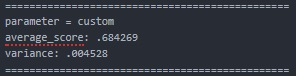
\includegraphics[width=12cm, bb=0 0 296 76]{optimal2.jpg}
		\end{center}
	\end{minipage}
	\begin{minipage}{0.50\hsize}
		\begin{center}
			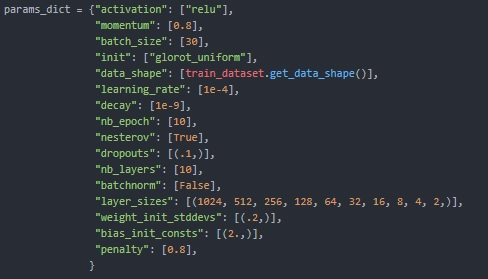
\includegraphics[width=12cm, bb=0 0 488 279]{optimal2p.jpg}
		\end{center}
	\end{minipage}
	\caption{一番良かったパラメーターとその実行結果}
	\label{optimal2}
\end{figure}

\clearpage

\section{MUVデータセットについて}

まず、このデータ・セットがなんのためにあるのかについて、論文\cite{thesis}を読んでわかったことを以下で説明する。


現代の薬学の世界では、バーチャールスクリーニングを行うことにより、薬学的に役に立つであろう物質を選び出すことが行われている。
ところが、最近の研究により分子構造に基づいたバーチャルスクリーニング(SBVS)は、バリデーションで用いられるデータセットが結果に大きな影響を及ぼすことがわかった。特に、データ・セット間で分子量・水素結合の数等の「シンプル」な性質が大きく異なっていると、スコアが上がったかのように見えることがわかっている。
したがって、ある一定の範囲に収まる「シンプル」な性質を持つものを集めたデータ・セットでなければ、正しいバリデーションとは言えず、バイアスがかかってしまうと考えられる。今回用意されているデータ・セットは、そのようなバイアスがかからないように、集められたものであり、これはMaximum Unbiased Validation(最もバイアスが小さいバリデーション)メソッドを用いたバーチャルスクリーニングを可能にする。


次に、データ・セットに含まれていたタンパク質のうちの一つに注目し、それに対して活性のある化合物と活性のない化合物を挙げる。
これらのデータは、PubChem\cite{MUV-600}より入手したものである。

今回注目したタンパク質は、MVUのデータ・セットに含まれる、MUV-600というものである。
MUV-600の構造は図\ref{muv-600-fig}のとおりになっている。

\begin{figure}[H]
	\begin{minipage}{0.5\hsize}
		\begin{center}
			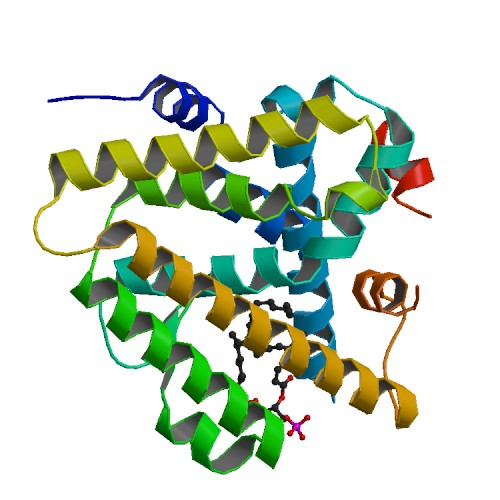
\includegraphics[width=12cm, bb=0 0 500 500]{../pictures/MUV-600/1.jpg}
		\end{center}
	\end{minipage}
	\begin{minipage}{0.5\hsize}
		\begin{center}
			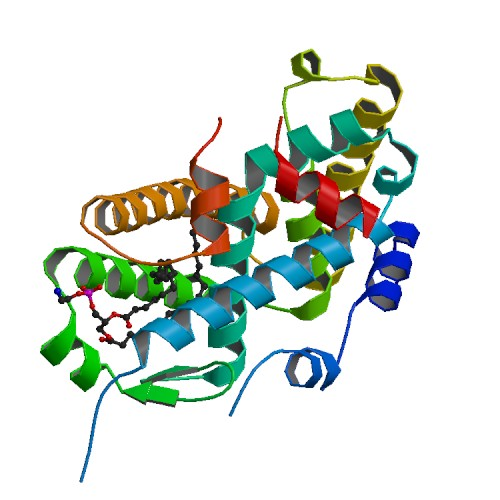
\includegraphics[width=12cm, bb=0 0 500 500]{../pictures/MUV-600/2.jpg}
		\end{center}
	\end{minipage}
	\\
	\begin{minipage}{0.5\hsize}
		\begin{center}
			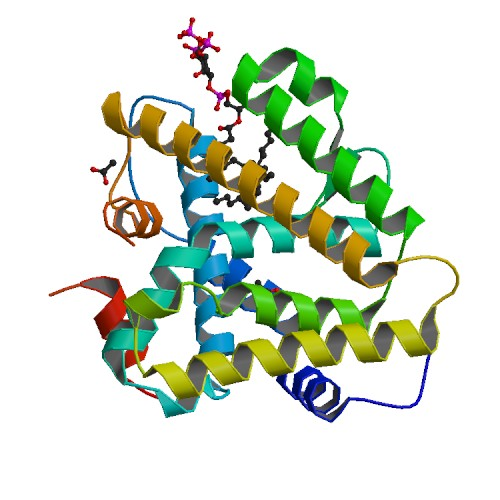
\includegraphics[width=12cm, bb=0 0 500 500]{../pictures/MUV-600/3.jpg}
		\end{center}
	\end{minipage}
	\begin{minipage}{0.5\hsize}
		\begin{center}
			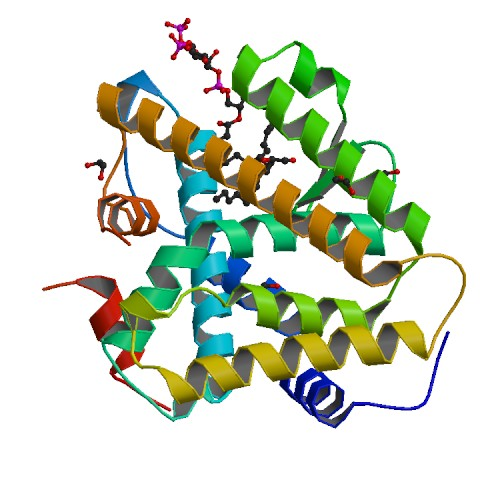
\includegraphics[width=12cm, bb=0 0 500 500]{../pictures/MUV-600/4.jpg}
		\end{center}
	\end{minipage}
	\caption{MUV-600の構造} \label{muv-600-fig}
\end{figure}

このタンパク質に対し、活性のある化合物として図\ref{active}のような構造をしているものが例として挙げられる。

\begin{figure}[H]
	\begin{minipage}{0.33\hsize}
		\begin{center}
			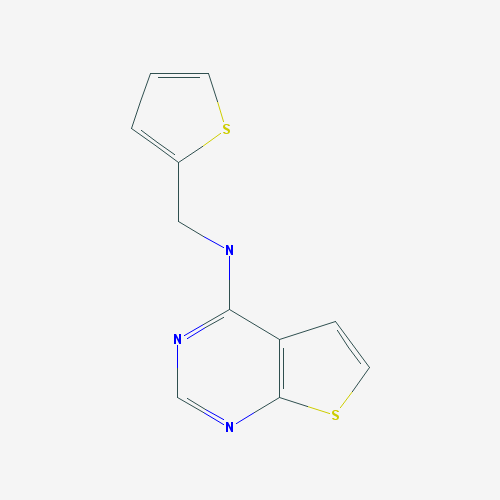
\includegraphics[width=7cm, bb=0 0 500 500]{../pictures/active/1.png}
		\end{center}
	\end{minipage}
	\begin{minipage}{0.33\hsize}
		\begin{center}
			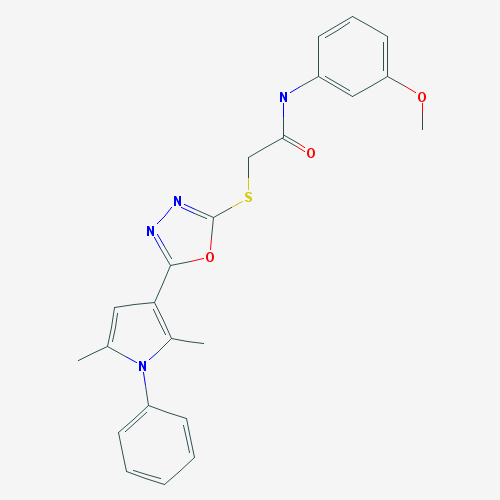
\includegraphics[width=7cm, bb=0 0 500 500]{../pictures/active/2.png}
		\end{center}
	\end{minipage}
	\begin{minipage}{0.33\hsize}
		\begin{center}
			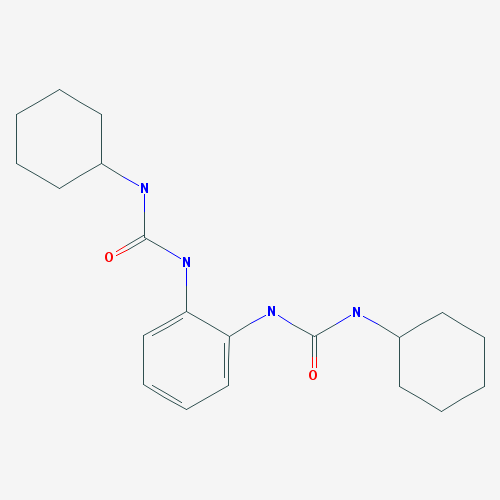
\includegraphics[width=7cm, bb=0 0 500 500]{../pictures/active/3.png}
		\end{center}
	\end{minipage}
	\caption{活性のある化合物} \label{active}
\end{figure}

一方、活性のない化合物としては図\ref{inactive}のようなものが挙げられる。

\begin{figure}[H]
	\begin{minipage}{0.33\hsize}
		\begin{center}
			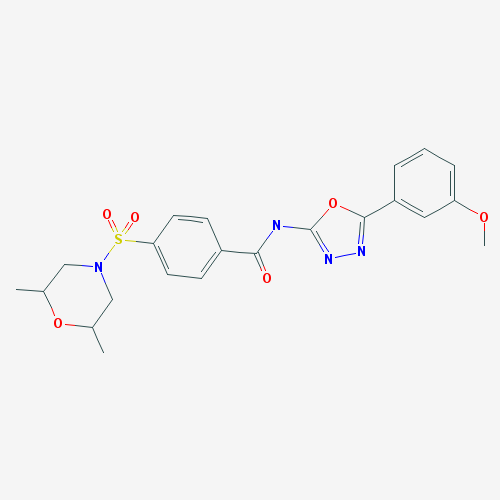
\includegraphics[width=7cm, bb=0 0 500 500]{../pictures/inactive/1.png}
		\end{center}
	\end{minipage}
	\begin{minipage}{0.33\hsize}
		\begin{center}
			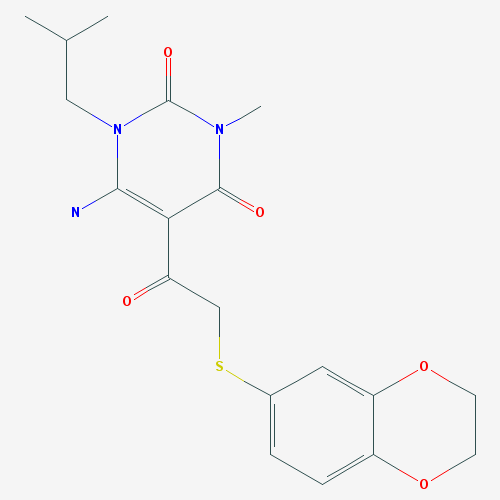
\includegraphics[width=7cm, bb=0 0 500 500]{../pictures/inactive/2.png}
		\end{center}
	\end{minipage}
	\begin{minipage}{0.33\hsize}
		\begin{center}
			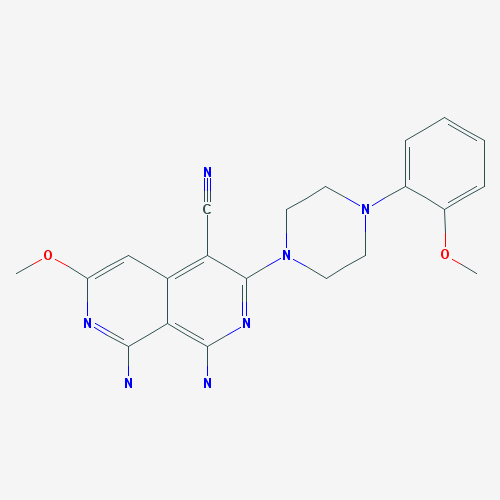
\includegraphics[width=7cm, bb=0 0 500 500]{../pictures/inactive/3.png}
		\end{center}
	\end{minipage}
	\caption{活性のない化合物} \label{inactive}
\end{figure}

\begin{thebibliography}{9}
	\bibitem{thesis} Sebastian G. Rohrer and Knut Baumann, "Maximum Unbiased Validation (MUV) Data Sets for Virtual Screening Based on PubChem Bioactivity Data, "  https://pubs.acs.org/doi/10.1021/ci8002649 as of Oct. 21 2018.
	\bibitem{MUV-600} PubChem MUV-600, \url{https://pubchem.ncbi.nlm.nih.gov/bioassay/600#section=Protocol} Protein Target: \url{https://pubchem.ncbi.nlm.nih.gov/target/protein/NP_004950} as of Oct. 21 2018
	\bibitem{regularization} 過学習を防ぐ方法, \url{https://products.sint.co.jp/aisia/blog/vol1-8} as of Oct. 21 2018
	\bibitem{epoch_batch} Difference between a batch and an epoch, \url{https://machinelearningmastery.com/difference-between-a-batch-and-an-epoch/} as of Oct. 22 2018
	\bibitem{momentum} Quora: What does momentum mean in neural network, \url{https://www.quora.com/What-does-momentum-mean-in-neural-networks} as of Oct. 22 2018
	\bibitem{lrd} Quora: What is learning rate in neural networks, \url{https://www.quora.com/What-is-the-learning-rate-in-neural-networks} as of Oct. 22 2018
	\bibitem{dropout} Quora: Why exactly does dropout in deep learning work, \url{https://www.quora.com/Why-exactly-does-dropout-in-deep-learning-work} as of Oct. 22 2018
	\bibitem{bs} StackExchange: What is weight and bias in deep learning, \url{https://datascience.stackexchange.com/questions/19099/what-is-weight-and-bias-in-deep-learning} as of Oct. 22 2018
	\bibitem{layernode} How to configure the number of layers and nodes in a neural network, \url{https://machinelearningmastery.com/how-to-configure-the-number-of-layers-and-nodes-in-a-neural-network/} as of Oct. 22 2018
\end{thebibliography}
\end{document}
